\section{Definition of a 3D display}
While it is commonplace to hear about 3D display in television or smartphone advertisement nowadays, the distinction between 2D and 3D might be more difficult to settle.
\subsection{The problem}
If we take the simple definition : a 3D display is a display that can show 3D images, it is really ambiguous, because of what is supposed to be "3D". For instance, for years, video games have been advertising 3D engines and spectacular 3D graphics, even without the depth provided by what is now called 3D displays or 3D movies in cinema.

Hence, we have to qualify what is 3D and what it is not.
\subsection{Parameters}
In the litterature (\cite{okoshi1976three}, \cite{pimenta2012comprehensive}), the main idea is to relate to the human brain and body capabilities to define 3D vision. For instance, a big part of the "3D" feel is due to the fact of having two eyes that looks in the same direction, but from a slightly different angle, but it is not the only parameter.

The visual cues of 3D vision are separated in two families:  
\begin{itemize}
\item Physiological cues. They will relate to the capabilities of the human body.
\item Psychological cues. They will relate to the information inference capabilities of the human brain.
\end{itemize}
\subsection{Presentation of common visual cues}

\begin{figure}[h!]
\centering
\begin{tabular}{|c|}
\hline
Psychological cues \\
\hline
\Gls{occlusion} \\
\Gls{linpersp} \\
\Gls{atmpersp} \\
\Gls{shading} \\
\hline
\end{tabular}
\caption{Psychological cues}
\end{figure}
\section{Classification of the 3D displays}
One of the main problem while trying to find a proper \gls{display} for a given application is to choose a relevant classification for the displays, that allows a choice with criterions relevant to the application.
\subsection{Criterions}
There was a lack of proper nomenclature in the literature for a long time \cite{pimenta2012comprehensive}. However, some attemps have been made to find relevant criterions that would be general enough to cover the current display techniques, but also the ones that are not yet thought of.

\subsubsection{Different classifications}
The first classification was in \cite{okoshi1976three}, and it was really based upon the different kinds of displays : 
\begin{itemize}
\item Lens-sheet three dimensional pictures.
\item Projection-type three dimensional displays.
\item Holography.
\end{itemize}

However, it did not hold well against the emergence of new techniques, like volumetric displays for instance.

Other classifications %\cite{ref nécessaire} 
would limit themselves to only a subset of 3D displays.

Hence the need for a classification that would not base itself on the different technologies, but on criterions that would be inherent to the idea of display and human vision.

\subsubsection{Chosen classification}
In \cite{pimenta2012comprehensive}, the main idea is to classify the displays according to two axes : 

\begin{itemize}
\item The display depth (flat or deep).
\item The number of points of view from which the image can be seen (duoscopic, multiscopic, or omniscopic).
\end{itemize}

\section{In-depth presentation of some 3D display methods}
This section describes the different technologies used by manufacturers of 3D displays, and also explains some 3D visualization systems in detail. But first we will define what are stereoscopic and auto-stereoscopic displays. \\
\textbf{Stereoscopy} is the set of techniques used to reproduce a depth perception from two planar images.\\
\textbf{Autostereoscopy} is a method of image representation, either in three-dimension or stereoscopic, which requires no additional device to render the 3D effect. 

\subsection{Two-view 3D displays}
Since a decade, a new generation of screens appeared: 3D screens. The main feature of these screens, which distinguishes them from conventional screens, is their ability to display stereoscopic images, : each eye of the observer will receive a different point of view.
There are multiple technologies that are able to power such screens; we will explain some. But an exhaustive list is present in \cite{mehrabi2013making}.

\subsubsection{Wavelength selective displays}
To view in 3D, it is necessary to provide our brain two images of the same scene taken from two different points of view. This is the principle of stereoscopy. The distance between the two points of view is used to compute the depth of field to achieve the 3D effect.\\
Different methods exist so that each eye receives the intended image. 

The most famous are the anaglyphic glasses (red and cyan glasses). However, the result is of poor quality.

\begin{figure}[h!]
\begin{center}
\begin{minipage}{1\linewidth}
\centering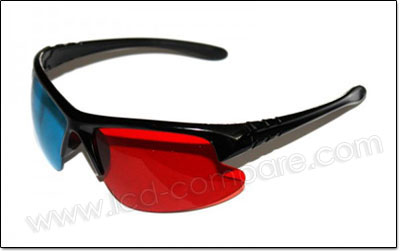
\includegraphics[width=6cm,height=40mm]{image/1.jpg}
\caption{Red/cyan color filter 3D Glasses\cite{ViewingOn3D}}
\end{minipage}
\end{center}
\end{figure}

In this case, images are filtered by color. The two images are superimposed and the glasses incorporate a color filter. The eyes can only see the image intended for them, so this can be used to create a stereoscopic effect. 

This is a passive method.

\subsubsection{Time-sequential two-view displays}
The idea is that the images are shown one after the other, but it has two requirements : 
\begin{itemize}
\item The switching between images must be fast : a refresh rate of 48 Hz is theoretically minimal for a 24 fps movie, however research \cite{holliman2011three} shown that 58 Hz is a practical minimum.
\item Each eye must see only the images directed to it. There are multiple technologies to achieve this, passive and active.
\end{itemize}

\paragraph{Passive method}
This technique uses polarized glasses. The right lens is polarized in one direction while the left lens is polarized in the other direction. 

\begin{figure}[h!]
\begin{center}
\begin{minipage}{1\linewidth}
\centering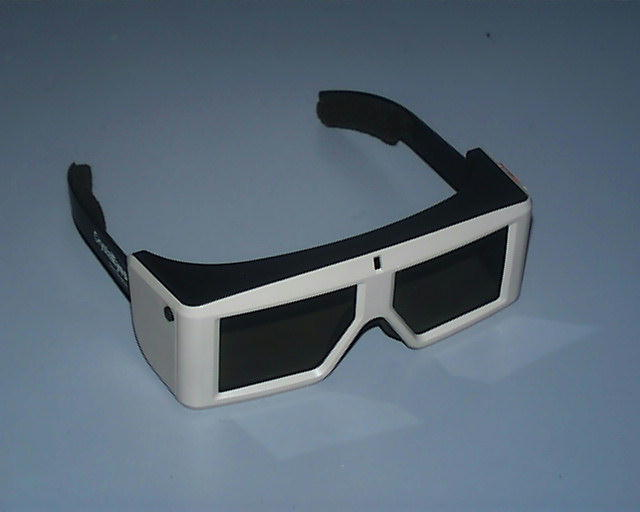
\includegraphics[width=6cm,height=30mm]{image/2.jpg}
\caption{Polarized 3D system\cite{Polarized3D}}
\end{minipage}
\end{center}
\end{figure}

This is not an expensive method, however the image is often less bright. It is generally used in movie theaters.

\paragraph{Active method}
This technique uses active glasses, with LCD shutters that needs to be synchronized with the screen refresh rate : one of the glass goes black while the other allow the light to pass, which allows the eyes to receive only the wanted image at the wanted time.

This method is more expensive, but reviews often said it offers a better experience.

\subsubsection{Time-parallel two-view displays}
This is the opposite of time-sequential two-view displays. Both eyes receive a stream of images at the same time.

\paragraph{Simple stereoscopy}
These displays use glasses and generate two simultaneous images. They include double projection systems that combine two projectors and polarizing filters matched with appropriate glasses.\\

\textbf{Advantages}
\begin{itemize}
\item The glasses are easy to build, and therefore widely available from suppliers.
\item The quality of the polarizer and the nature of the polarization retention screens are important.
\end{itemize}

%\newline
\paragraph{Auto-stereoscopy}
This technique provides a terrain vision without wearing glasses adjusted, the observer is placed at the correct distance from the screen, with each eye sees the image that corresponds to it (an image will be sent to the right eye and another to the left eye and the brain will add recreating the effect of relief).\\
\textbf{The disadvantages:}
\begin{itemize}
\item He must be placed precisely over the screen, if the observer is not the precise position relative to the screen he will see superimposed images and is unreadable.
\item The system is also tiring for the eyes.
\item He does not allow the visualization of the stereoscopic image to multiple viewers at the same time.
\end{itemize}

%%%%%%%%%%%%%%%%%%%%%%%%%%%%%%%%%%%%

\subsection{Horizontal paralax multiview 3D diplays} 

There are two main types of technology for Multiview parallax displays: Or by applying a parallax barrier,or by application of a lenticular panel.\\
A parallax barrier is a mask of parallel black stripes that reveals the different parts of the underlying image depending on the direction of observation.\\ The same effect can be obtained with the lenticular sheets, which are linear networks of narrow cylindrical lenses. Both techniques are used to show a unique view of each position in the viewing area.Thus, a viewer feels the motion parallax and binocular stereo without the use of special glasses. 

\subsubsection{Lenticular Displays}

The application of a lenticular panel to deflect the rays from the pixels of the screen in order to reproduce a stereoscopic display giving the late images giving an impression of relief (3D).\\ Lenticular panel is composed of a regular grid of small spherical lenses.Each lens covers an area of several pixels of the flat screen and will divert the direction of the light emitted by the pixels covered.\\
Thus the principle according to the imaging angle of view we see the red image or the blue image. An observer looking at a lens 3D screen does not see the same screen pixel flat between his left eye and his right eye, although both eyes set the same lens.\\
On the figure below, the left eye sees a lens emitting red color (from a red pixel) while the right eye sees simultaneously the same lens blue.\\
With horizontal lenses, projecting changing images, the image is seen depending on the viewing angle of the lens.

\begin{figure}[h!]
\begin{center}
\begin{minipage}{1\linewidth}
\centering
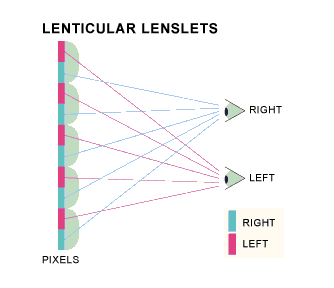
\includegraphics[width=8cm,height=5cm]{image/lentuc.png}
\caption{A lens array\cite{glasses-free3D}}
\end{minipage}
\end{center}
\end{figure}

\subsubsection{Parallax Barrier Displays}

Each cache is precisely placed so that the observer, itself placed at the correct distance from the screen, with each eye sees the image that corresponds to it. The images are divided into columns of a pixel wide. Thanks to the cache and inserting columns of each image, an image is sent to the right eye and one in the left eye and the brain will add recreating the relief effect.\\
In comparison with the lens array, we can see each spherical lens replaced by an opaque surface and a small hole in its center. Therefore, as in the case of the lens array, an observer looking at a small hole in the 3D screen does not see the same screen pixel flat between his left eye and his right eye: this is because the barrier parallax is not contiguous to the flat screen, a distance of a few millimeters between the two panels.\\
On the figure below, the left eye sees through a hole in a red color (from a red pixel) while the right eye sees a blue simultaneously through the same hole.
\clearpage

\begin{figure}[h!]
\begin{center}
\begin{minipage}{1\linewidth}
\centering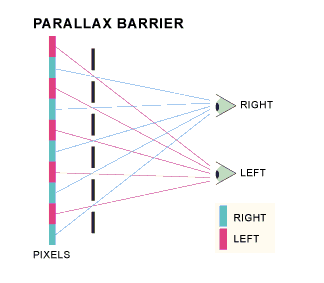
\includegraphics[width=8cm,height=5cm]{image/parallax.png}
\caption{A parallax barrier\cite{glasses-free3D}}
\end{minipage}
\end{center}
\end{figure}

This technique provides a terrain vision without wearing glasses.\\

\textbf{The disadvantages:}
\begin{itemize}
\item It must be placed precisely over the screen, if the observer is not the precise position relative to the screen he will see superimposed images and is unreadable.
\item We are not machines and we move without us realizing what is not compatible with the system.
\item It does not allow visualization of the stereoscopic image to multiple viewers at the same time.
\end{itemize}

\subsubsection{Multi-Projector Displays:}

This technique consists of positioning in a circle several projectors displaying all an angle different image after these images are projected onto a special screen, double lenticular lens example (spherical lens), the easiest way to project these images on a cylinder fog.

\begin{figure}[h!]
\begin{center}
\begin{minipage}{1\linewidth}
\centering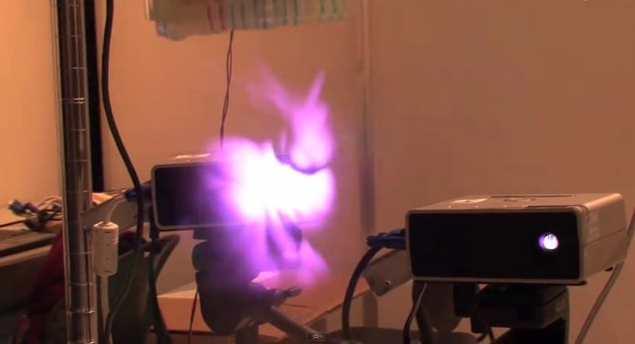
\includegraphics[width=6cm,height=4cm]{image/lapin.png}
\caption{3D multiviewpoint display\cite{3Dmultiviewpoint}}
\end{minipage}
\end{center}
\end{figure}

It is possible to turn around the rabbit in 3 dimensions and view it from all angles.\\
\textbf{The advantage:} 

\begin{itemize}
\item One advantage of this technique, the size of the 3D image may be much larger, there is currently no limit.
\end{itemize}
\textbf{The disadvantages:}
\begin{itemize}
\item  Multiple projectors are needed (for projector).
\item Headlights must be precisely aligned.
\end{itemize}


%%%%%%%%%%%%%%%%%%%%%%%%%%%%%%%%%%%%%%%%%
\subsubsection{Pepper's Ghost}
\subsubsection{Glasses}
\subsubsection{Head-mounted displays}
\subsubsection{Hologram}
\subsubsection{Autostereoscopic screen}
% En rajouter à volonté